\documentclass[10pt]{article}
\usepackage{listings}
\usepackage{graphicx}
\usepackage{verbatim}
\usepackage{float}
\begin{document}
\title{CS 378: Final Project}
\author{Sai Avala \\ Vaibhav Gupta \\ Sudheesh Katkam}
\date{December 10, 2014}
\maketitle
\section{Introduction}
\label{introduction}
\sf For this project we wanted to work on a system of linear equations solver. There are various ways
of solving a system of linear equations, but for this project we decided to work on the
\textit{Jacobi Algorithm}. The way the Jacobi algorithm works is by the choosing a simple solution,
and then increasing the number of iterations until you converge to a certain solution. At this point
that converged solution should hopefully be the correct answer. There might be a minor error,
but this can be controlled by you. The first part of this project was to implement the regular
iterative solution to the Jacobi algorithm. We then went ahead and used OpenMP to parallelize it
and also vectorized parts of the implementation to further increase the speedup. In addition to 
implementing a hybrid parallelized and vectorized solution, we also used Valgrind and Gprof
in order to profile our code and then improve our solutions. As for reference, our algorithms
are optimized for dense matrices.

\section{The Algorithm}
\label{algorithm}
\sf Here we will describe the basic algorithm. Lets take the standard system of linear equations,
Ax = b. We are given matrix A, and the vector b, but want to solve for x. The way the iterative
Jacobi algorithm works is by first assuming a solution and then iterating until we've converged
to an error point. The way we do this is by understanding that matrix A can be rewritten as
A = D + L + U, where D is the diagonalization matrix and L + U is the summation of the LU
factorization. We can then reaarange the formula such that x\_(i+1) = D(inverse)*(b - (L + U)x).

\section{Results}
\label{results}
\sf A couple of our results are below:
\begin{figure}[H]
    \centering
    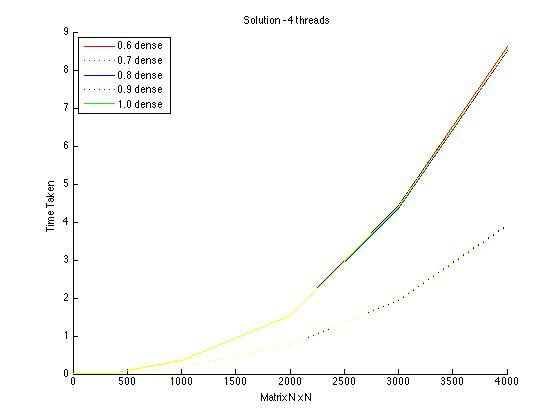
\includegraphics[width=\textwidth]{density-4threads}
    \caption{Varying density of the matrix, outputs runtime}
\end{figure}
\sf The figure above shows the runtime while varying the density of the matrices. The dotted
lines represent matrices that use the vectorized solution and the solid lines are those that
don't use the vectorized implementation. As you can see, when we turn on vectorization,
we get a significant performance boost. The figure above was run on only 4 thread.
\begin{figure}[H]
    \centering
    \includegraphics[width=\textwidth]{threads-07dense}
    \caption{Varying number of threads amongst density}
\end{figure}
\sf The figure above shows the runtime when varying the number of threads amongst a 70\%
dense matrix. As you can see, as the number of threads increases, we improve in runtime.
We further improve in runtime when we turn on vectorization as well (the dotted lines) in
addition to the multithreading.

\section{Profiling}
\label{profiling}
\sf While working on this project we used Valgrind and Gprof to help guide us when working
on the performance boosts. Valgrind was able to provide information regarding memory usage
in the program. We noticed that there was some error in branch prediction, but this is
most likely due to using OpenMP. We didn't have an error in branch prediction prior
to using OpenMP. We used Gprof to note what function took the most time and was the
most expensive for us. By using Gprof, we noticed that generating small matrices
took a very long time. However as the matrices increased in size, matrix generation
didn't take as long. Our use of frand() generally took awhile, because we had to generate
random floating number to fill in the matrix. Calculating error took a long time,
however we ended up not optimizing this. In addition, we used Gprof to verify that
our use of vectorization was actually more optimal than a standard iterative solution.
In addition, we used Gprof to minimize general stack usage. 

\section{Challenges}
\label{challenges}
\sf While working on this project we did run into a couple challenges. In the beginning,
we had an issue where our solution wasn't converging in fast enough iterations. What
we mean by this is that our solution should have converged at maybe 10 iterations rather than 86
iterations. This was a minor issue that we could solve. The main point of interest is how we handlded
vectorization and multithreading. We originally used C++11 threads, but to make everything more
straightforward in terms of synchronization, we used OpenMP. Our challenge with completing the
vectorization was in making sure that computations (for the results) were still the same. Because
we were working with heavy floating point numbers, we had to avoid the issue of some small
floating point arithmetic error.

\section{Future Work}
\label{futureWork}
\sf Currently this project uses OpenMP and Intel SSE intrinsics for vectorization. OpenMP
is a multithreading framework which makes use of shared memory. However, if we were to take
this project further, we would want to try to use MPI. MPI is a message passing interface
which allows us to do multicore processing amongst distributed memory. By using MPI,
we would want to see if there is even more significant speedups.


\end{document}
